\section{\ref{rq:finding-changes} How can we find changes between two models?}

Finding changes it handled in the \verb|Testar.ChangeDetection.Core.Algorithm| namespace. Since it is in the \verb|Testar.ChangeDetection.Core| assembly various applications can use the algorithm and therefore it is not a UI feature only. The visualisation of the differences are handled by the new analysis website and discussed in section \ref{rq:type-visualisation-answer}

The classes used for the algorithm are visualised in Figure \ref{fig:class-diagram-differences}. For visibility purposes the interfaces are omitted.

\begingroup
\captionsetup{type=figure}
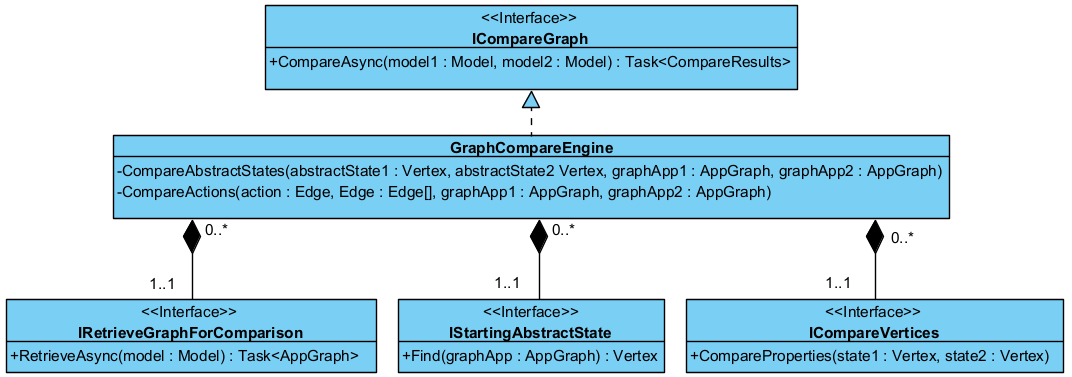
\includegraphics[scale=0.5]{thesis/images/4-UML-Differences.png}
\captionof{figure}{Class diagram differences (UML 2.0)}\label{fig:class-diagram-differences}
\endgroup

\subsection{The change detection algorithm}

The core of the algorithm is implemented by the \verb|GraphCompareEngine| class. The \verb|CompareAsync| method is given two app models, \verb|model1| and \verb|model2|. Before models can be compared, each graph need to be retrieved. The retrieval process is handled by the \verb|GraphForCompareRetriever| class. For the algorithm only need the data from the Abstract Layer, the Concrete Layer and the Abstract Concrete connectors.



% TODO give brief summary to explain terminology like corresponding states, walk over actions etc. 

The second step of the algorithm is the determining where to start the change detection. This can be 

Due to the nature of the algorithm, explained later in this section, it needs to known where to start. This task is implemented by the \verb|InitialStartingAbstractState| class. For now it is assumed that the initial abstract state are corresponding states. Different starting strategies can be implemented by implementing the \verb|IStartingAbstractState| interface. 




%Abstract Graph comparison
%First the software create a ComparableGraph. A Comparable graph only contacts the nodes and edges from the abstract states and abstract actions. The data however will include data from the concrete states and actions. 

%When we have a changed abstractstate, get a widgettree of one concrete state
%https://www.xmlunit.org/  have a package for both java as .NET to create differences between version.

%using a fast mode
%the fast mode will only look into changes on the abstract level. Changes like different colours for example



for the graph only the Abstract Layer, the concrete Layer and the Abstract Concrete connectors are using. 

% Every element has an ID generated by OrientDb e.g. #154:0. When merging elements those Id's are merged to by the following algorithm: \#Id1\_Id2 e.g. \#150:0\_\#150:1. 

difference engine
merge graph \cite{andrews2009visual}
the graph needs to be similar are "enough"

Finding matching notes is done by the difference algorithm. 




\subsection{Calibration}
\subsection{Difference Engine}
\subsection{Difference Graph}
